\documentclass{report}
\usepackage{hyperref}
\usepackage{tikz}
\title{Fake News Detection using NLP and Deep Learning}
\author{TODO: Author Name}
\date{\today}
\begin{document}
\maketitle
\begin{abstract}
TODO: Abstract content.
\end{abstract}
\tableofcontents
\chapter{Introduction}
TODO: Introduction text.
\chapter{Literature Review}
TODO: Literature review text.
\chapter{Methodology}
The workflow for detecting fake news is illustrated in Figure~\ref{fig:pipeline}.

\begin{figure}[h]
    \centering
    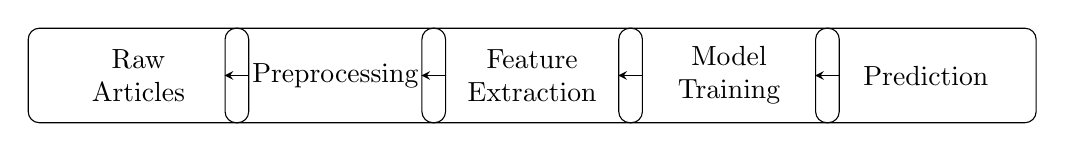
\begin{tikzpicture}[
        node distance=2.5cm,
        >=stealth,
        every node/.style={draw, rectangle, rounded corners, align=center, minimum width=2.8cm, minimum height=1.2cm}
    ]
        \node (data) {Raw\\Articles};
        \node (prep) [right of=data] {Preprocessing};
        \node (feat) [right of=prep] {Feature\\Extraction};
        \node (model) [right of=feat] {Model\\Training};
        \node (pred) [right of=model] {Prediction};

        \draw[->] (data) -- (prep);
        \draw[->] (prep) -- (feat);
        \draw[->] (feat) -- (model);
        \draw[->] (model) -- (pred);
    \end{tikzpicture}
    \caption{Processing pipeline used in this project.}
    \label{fig:pipeline}
\end{figure}

TODO: Methodology details.
\chapter{Experiments}
TODO: Experiments and results.
\chapter{Discussion}
TODO: Discussion.
\chapter{Conclusion}
TODO: Conclusion.
\bibliographystyle{plain}
\bibliography{refs}
\end{document}
